\documentclass[t,aspectratio=169,10pt]{beamer}

\usepackage[utf8]{inputenc}

\usepackage{amsmath}
\usepackage{mathastext}
\usepackage{multicol}
\usepackage{multirow}
\usepackage{textcomp} % to use \textmu
\usepackage[absolute,overlay]{textpos} % to place floating text boxes with \begin{textblock*}{width}(x,y)
\usepackage{tcolorbox}

\usepackage{tikz}
\usetikzlibrary{decorations.pathreplacing}
\usepackage{circuitikz}

\usepackage{graphicx}
\graphicspath{{./figuras/}}

\setbeamertemplate{navigation symbols}{}

\title{Clase 13}
\subtitle{El transistor MOSFET}
\author{Dr.-Ing. Juan José Montero Rodríguez}
\subject{Elementos Activos}
\institute{Escuela de Ingeniería Electrónica}
\date{Semestre I-2024}
\titlegraphic{
\includegraphics[height=8mm]{logotec.pdf}}


\begin{document}

\begin{frame}
\titlepage
\end{frame}


\section{Introducción}
\begin{frame}{Transistor MOSFET}

Transistor: dispositivo de al menos tres terminales, en el que una terminal controla el flujo de corriente entre las otras dos

%\includegraphics[width=11cm]{acronimos}

\centering
\vspace{5mm}
\textbf{Transistor: transfer resistor}

\vspace{5mm}
\textbf{MOSFET: metal-oxide-semiconductor field-effect transistor}

\raggedright
\vspace{5mm}
MOSFETs

\begin{itemize}
\item Basado en el principio de efecto de campo
\item Uso de un campo eléctrico para controlar corriente entre dos terminales
\item Transistor más utilizado (más de 80\% del mercado)
\item Base de la industria microelectrónica
\end{itemize}
\end{frame}


\begin{frame}{Historia del MOSFET}

\begin{itemize}
	\item Principio de efecto de campo presentado en 1925 por Julius Lillienfeld
	\begin{itemize}
		\item Patente de MOSFET presentada en 1928 por Lillienfeld
		\item Implementación posible en los 60s
	\end{itemize}
	\item Teoría de escalamiento = miniaturización
\end{itemize}

\vspace{3mm}\centering
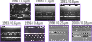
\includegraphics[width=11cm]{crosssections}
\end{frame}


\begin{frame}{Simbología del MOSFET}

\begin{itemize}
\item Símbolos de tres terminales: flecha indica la dirección de la corriente.
\item Símbolos de cuatro terminales: flecha en substrato apunta de P a N.
\end{itemize}

\begin{columns}

	\begin{column}{0.5\textwidth}
 	
		\begin{figure}[H]
		  \centering
            \begin{circuitikz}[arrowmos,nocircle]
                \draw (0,0) node[nmos](nmos1){};
                \draw (0,-1.5) node[]{NMOS};
                \draw (nmos1.drain) node[above]{D};
                \draw (nmos1.source) node[below]{S};
                \draw (nmos1.gate) node[left]{G};
                \draw (3,0) node[pmos](pmos1){};
                \draw (pmos1.source) node[above]{S};
                \draw (pmos1.drain) node[below]{D};
                \draw (pmos1.gate) node[left]{G};
                \draw (3,-1.5) node[]{PMOS};
            \end{circuitikz}
		\end{figure}
  
	\end{column}
 
	\begin{column}{0.5\textwidth}

        \begin{figure}[H]
		  \centering
            \begin{circuitikz}[arrowmos,nocircle]
                \draw (0,0) node[nfet](nmos1){};
                \draw (0,-1.5) node[]{NMOS};
                \draw (nmos1.drain) node[above]{D};
                \draw (nmos1.source) node[below]{S};
                \draw (nmos1.gate) node[left]{G};
                \draw (nmos1.bulk) node[right]{B};
                \draw (3,0) node[pfet](pmos1){};
                \draw (pmos1.source) node[above]{S};
                \draw (pmos1.drain) node[below]{D};
                \draw (pmos1.gate) node[left]{G};
                \draw (pmos1.bulk) node[right]{B};
                \draw (3,-1.5) node[]{PMOS};
            \end{circuitikz}
		\end{figure}

        \end{column}
 
\end{columns}

\vspace{5mm}
\begin{itemize}
    \item Las cuatro terminales del dispositivo son G (gate, compuerta), D (drain, drenador), S (source, fuente) y B (bulk, substrato).
    \item En el símbolo de tres terminales, el sustrato está conectado con la fuente.
    \item La tensión de la compuerta $V_G$ controla el flujo de corriente de drenador $I_D$.
\end{itemize}

\end{frame}


\begin{frame}{Efecto de campo en el condensador MOS}

La figura muestra un condensador MOS.

\begin{itemize}
    \item Metal: placa conductora, también puede ser de polisilicio fuertemente dopado.
    \item Óxido: aislante, tradicionalmente dióxido de silicio ($SiO_2$), dióxido de hafnio ($HfO_2$).
    \item Semiconductor: oblea de silicio, dopada tipo p.
\end{itemize}

\begin{figure}[H]
    \centering
    \includegraphics[width=0.8\textwidth]{figuras/condensador_mos.png}
\end{figure}

Funcionamiento:

\begin{itemize}
    \item El potencial de la compuerta permite controlar la concentración de portadores en el canal.
    \item La carga aplicada a la compuerta es igual a la carga almacenada en el canal.
    \item En el canal, el dopado efectivo es función de la tensión aplicada a la compuerta.
\end{itemize}
    
\end{frame}


\section{Estructura}
\begin{frame}{Corte transversal del MOSFET}

\centering
\includegraphics[width=11cm]{transistor1}

\raggedright
\begin{itemize}
	\item Dispositivo de 4 terminales: compuerta, fuente, drenador y substrato
	\item Dispositivo UNIPOLAR $\Rightarrow$ corriente de conducción involucra prácticamente sólo un tipo de portador de carga
	\item MOSFET consiste en
	\begin{itemize}
		\item dos regiones semiconductoras fuertemente dopadas separadas por una región semiconductora de tipo complementario
		\item un aislante y un electrodo sobre dicha región
	\end{itemize}
\end{itemize}

\end{frame}

\begin{frame}{Estructura del MOSFET}

\centering
\includegraphics[width=11cm]{transistor2}

\end{frame}


\begin{frame}{Transistores NMOS y PMOS}
	\begin{columns}
		\begin{column}{0.5\textwidth}
			\centering
			\includegraphics[width=5cm]{NMOS}
			
			\raggedright
			\begin{itemize}
				\item Flujo de corriente: de drenador a fuente
				\item Drenador es región n+ conectada al potencial más alto
				\item Se forma canal tipo N entre drenador y fuente
				\item Flujo de corriente debido a electrones
			\end{itemize}
		\end{column}
		\begin{column}{0.5\textwidth}
			\centering
			\includegraphics[width=5cm]{PMOS}
			
			\raggedright
			\begin{itemize}
				\item Flujo de corriente: de fuente a drenador
				\item Drenador es región p+ conectada al potencial más bajo
				\item Se forma canal tipo P entre drenador y fuente
				\item Flujo de corriente debido a huecos
			\end{itemize}
		\end{column}
	\end{columns}

\centering\vspace{2mm}
Desde el punto de vista de fabricación, la fuente y el drenador son intercambiables. Sólo pueden distinguirse después de polarizarlos

\end{frame}


\begin{frame}{Polarización del Substrato}
\begin{itemize}
	\item Diodos parásitos difusión-substrato deben estar polarizados en inversa
\end{itemize}

\vspace{3mm}
\centering
\includegraphics[width=11cm]{polsub}

\vspace{3mm}
\begin{itemize}
	\item NMOS: Substrato debe conectarse al voltaje más bajo del sistema, por ejemplo GND.
	\item PMOS: Substrato debe conectarse al voltaje más alto del sistema, por ejemplo V\textsubscript{DD}.
	\item También como protección ante el efecto de enganche (latch-up)
\end{itemize}
\end{frame}



\section{Funcionamiento}
\begin{frame}{Funcionamiento: Acumulación}

Acumulación: \hspace{5mm} $V_{GS} < 0$

\begin{itemize}
    \item Huecos se acumulan en la superficie
    \item No se forma canal entre drenador y fuente = transistor inactivo
    \item Sin canal $\Rightarrow$ MOSFET = Dos diodos en serie en direcciones opuestas $\Rightarrow$ I\textsubscript{DS} $\approx$ 0
\end{itemize}

\begin{figure}[H]
    \centering
    \includegraphics[width=7cm]{acumula1}
\end{figure}
 
 \end{frame}


\begin{frame}{Funcionamiento: Agotamiento}

Agotamiento: \hspace{5mm} $0 < V_{GS} < V_{TH}$

\begin{itemize}
    \item Huecos repelidos de la superficie = empobrecimiento de huecos en la superficie
    \item Transistor aún inactivo = región de subumbral
\end{itemize}

\begin{figure}[H]
    \centering
    \includegraphics[width=7cm]{agota1}
\end{figure}

\end{frame}


\begin{frame}{Funcionamiento: Inversión}

Inversión:\hspace{1cm} $V_{GS} \geq V_{TH}$

\begin{itemize}
	\item Electrones atraídos a la superficie = concentración de electrones en la superficie iguala concentración de huecos en el substrato $\Rightarrow$ Superficie de substrato p se comporta como material n
	\item Existe un canal entre drenador y fuente, transistor activo
\end{itemize}

\begin{figure}[H]
    \centering
    \includegraphics[width=7cm]{inversion1}
\end{figure}

\end{frame}


\section{Bandas}
\begin{frame}{Sistema Metal Óxido Semiconductor}
\centering
\includegraphics[width=11cm]{sistemaMOS}

El comportamiento del MOSFET se define con base en el POTENCIAL DE SUPERFICIE $\psi_S$ , que mide la deformación de bandas del semiconductor en la interfaz con el óxido
\end{frame}


\begin{frame}{Diagramas de bandas según $V_{GS}$}

\begin{figure}[H]
    \centering
    \includegraphics[width=0.8\textwidth]{figuras/bandas_mosfet.png}
\end{figure}
    
\end{frame}


\begin{frame}{Tensión de umbral}

El semiconductor tipo p originalmente tiene un dopado proporcional a:

    \[ \phi_F = E_i - E_F \]

Para lograr la inversión, se debe aplicar un potencial de superficie que logre eliminar el dopado tipo p y además agregar suficiente dopado tipo n:

    \[ \phi_S = 2\phi_F \]

La tensión de umbral se define como:

    \[ \boxed{ V_{TH} = \phi_{MS} + 2\phi_F + \dfrac{Q_{dep}}{C_{ox}} } \]

Donde $\phi_{MS}$ es la diferencia en las funciones de trabajo entre el polisilicio y el silicio de substrato, $\phi_F = (kT/q \ln (N_A / n_i))$ es la diferencia entre el nivel de Fermi y el intrínseco, $Q_{dep}$ es la carga almacenada en la región de agotamiento, y $C_{ox}$ es la capacitancia por unidad de área del óxido de compuerta.    
\end{frame}


\begin{frame}{Capacitancia de compuerta}

La carga almacenada en la estructura MOS es función de la tensión de la compuerta.

\begin{itemize}
    \item Varactor: condensador variable controlado por tensión.
\end{itemize}

\begin{figure}[H]
    \centering
    \includegraphics[width=0.5\textwidth]{figuras/mosfet_capacitance.png}
\end{figure}
    
\end{frame}


\begin{frame}{Lecturas recomendadas}

\begin{itemize}
    \item Razavi, B. (2013). Fundamentals of microelectronics. Chapter 6: Physics of MOS transistors, 2nd ed., pp. 270-288, Wiley.
\end{itemize}

\end{frame}

\end{document}
